% !TEX program = latexmk
% !TEX options = --output-directory=output "%DOC%"
\documentclass[12pt,a4paper,uplatex,dvipdfmx]{jsarticle}

% !TEX root = 20191106-Tatsuoka.tex
\usepackage{amsmath,amsfonts,amssymb}
\usepackage{amsthm}

\usepackage[T1]{fontenc}
\usepackage[uplatex,deluxe]{otf}
\usepackage[haranoaji]{pxchfon}
\usepackage{lmodern}
\usepackage{helvet}
\usepackage{bm}

\usepackage{thmtools}
\declaretheoremstyle[%
  headfont=\bfseries\sffamily,
]{sansserif}
\declaretheorem[name=定理, style=sansserif]{theorem}
\declaretheorem[name=定義, style=sansserif, sharenumber=theorem]{definition}
\declaretheorem[name=命題, style=sansserif, sharenumber=theorem]{proposition}
\declaretheorem[name=補題, style=sansserif, sharenumber=theorem]{lemma}
\declaretheorem[name=系, style=sansserif, sharenumber=theorem]{corollary}
\declaretheoremstyle[
  headfont=\bfseries\sffamily, 
]{sanserifproof}
\let\proof\relax
\declaretheorem[name={証明}, style=sanserifproof, unnumbered]{proof}
% \newtheoremstyle{sansserif}{}{}{}{}{\sffamily}{.}{ }{}
% \theoremstyle{sansserif}
% \newtheorem{theorem}{定理}
% \newtheorem{definition}[theorem]{定義}
% \newtheorem{proposition}[theorem]{命題}
% \newtheorem{lemma}[theorem]{補題}
% \newtheorem{corollary}[theorem]{系}
% \renewcommand{\proofname}{{\sffamily 証明}}
% \renewcommand{\qedsymbol}{$\blacksquare$}


\usepackage{mathtools}
\mathtoolsset{showonlyrefs=true}
\usepackage{geometry}
\geometry{truedimen,a4paper,hmargin=15mm,vmargin=20mm}
\usepackage{graphicx}
\usepackage{algorithm,algpseudocode}
\usepackage{hyperref}
\hypersetup{
  hidelinks=true,
  pdftitle={行列対数関数のための二重指数関数型公式の収束率について},
  pdfauthor={立岡文理,曽我部知広,剱持智哉,張紹良},
}
\special{dvipdfmx:config g 1.1}
\usepackage{pxjahyper}
\usepackage{titlesec}
\titleformat{\section}{\Large\sffamily\bfseries}{\thesection}{1em}{}
\titleformat{\subsection}{\large\sffamily\bfseries}{\thesubsection}{1em}{}
\titleformat{\subsubsection}{\normalsize\sffamily\bfseries}{\thesubsubsection}{1em}{}

% mathbb
\newcommand{\bba}{\mathbb{a}}
\newcommand{\bbb}{\mathbb{b}}
\newcommand{\bbc}{\mathbb{c}}
\newcommand{\bbd}{\mathbb{d}}
\newcommand{\bbe}{\mathbb{e}}
\newcommand{\bbf}{\mathbb{f}}
\newcommand{\bbg}{\mathbb{g}}
\newcommand{\bbh}{\mathbb{h}}
\newcommand{\bbi}{\mathbb{i}}
\newcommand{\bbj}{\mathbb{j}}
\newcommand{\bbk}{\mathbb{k}}
\newcommand{\bbl}{\mathbb{l}}
\newcommand{\bbm}{\mathbb{m}}
\newcommand{\bbn}{\mathbb{n}}
\newcommand{\bbo}{\mathbb{o}}
\newcommand{\bbp}{\mathbb{p}}
\newcommand{\bbq}{\mathbb{q}}
\newcommand{\bbr}{\mathbb{r}}
\newcommand{\bbs}{\mathbb{s}}
\newcommand{\bbt}{\mathbb{t}}
\newcommand{\bbu}{\mathbb{u}}
\newcommand{\bbv}{\mathbb{v}}
\newcommand{\bbw}{\mathbb{w}}
\newcommand{\bbx}{\mathbb{x}}
\newcommand{\bby}{\mathbb{y}}
\newcommand{\bbz}{\mathbb{z}}
\newcommand{\bbA}{\mathbb{A}}
\newcommand{\bbB}{\mathbb{B}}
\newcommand{\bbC}{\mathbb{C}}
\newcommand{\bbD}{\mathbb{D}}
\newcommand{\bbE}{\mathbb{E}}
\newcommand{\bbF}{\mathbb{F}}
\newcommand{\bbG}{\mathbb{G}}
\newcommand{\bbH}{\mathbb{H}}
\newcommand{\bbI}{\mathbb{I}}
\newcommand{\bbJ}{\mathbb{J}}
\newcommand{\bbK}{\mathbb{K}}
\newcommand{\bbL}{\mathbb{L}}
\newcommand{\bbM}{\mathbb{M}}
\newcommand{\bbN}{\mathbb{N}}
\newcommand{\bbO}{\mathbb{O}}
\newcommand{\bbP}{\mathbb{P}}
\newcommand{\bbQ}{\mathbb{Q}}
\newcommand{\bbR}{\mathbb{R}}
\newcommand{\bbS}{\mathbb{S}}
\newcommand{\bbT}{\mathbb{T}}
\newcommand{\bbU}{\mathbb{U}}
\newcommand{\bbV}{\mathbb{V}}
\newcommand{\bbW}{\mathbb{W}}
\newcommand{\bbX}{\mathbb{X}}
\newcommand{\bbY}{\mathbb{Y}}
\newcommand{\bbZ}{\mathbb{Z}}

% mathbf
\newcommand{\bfa}{\mbfa}
\newcommand{\bfb}{\mbfb}
\newcommand{\bfc}{\mbfc}
\newcommand{\bfd}{\mbfd}
\newcommand{\bfe}{\mbfe}
\newcommand{\bff}{\mbff}
\newcommand{\bfg}{\mbfg}
\newcommand{\bfh}{\mbfh}
\newcommand{\bfi}{\mbfi}
\newcommand{\bfj}{\mbfj}
\newcommand{\bfk}{\mbfk}
\newcommand{\bfl}{\mbfl}
\newcommand{\bfm}{\mbfm}
\newcommand{\bfn}{\mbfn}
\newcommand{\bfo}{\mbfo}
\newcommand{\bfp}{\mbfp}
\newcommand{\bfq}{\mbfq}
\newcommand{\bfr}{\mbfr}
\newcommand{\bfs}{\mbfs}
\newcommand{\bft}{\mbft}
\newcommand{\bfu}{\mbfu}
\newcommand{\bfv}{\mbfv}
\newcommand{\bfw}{\mbfw}
\newcommand{\bfx}{\mbfx}
\newcommand{\bfy}{\mbfy}
\newcommand{\bfz}{\mbfz}
\newcommand{\bfA}{\mbfA}
\newcommand{\bfB}{\mbfB}
\newcommand{\bfC}{\mbfC}
\newcommand{\bfD}{\mbfD}
\newcommand{\bfE}{\mbfE}
\newcommand{\bfF}{\mbfF}
\newcommand{\bfG}{\mbfG}
\newcommand{\bfH}{\mbfH}
\newcommand{\bfI}{\mbfI}
\newcommand{\bfJ}{\mbfJ}
\newcommand{\bfK}{\mbfK}
\newcommand{\bfL}{\mbfL}
\newcommand{\bfM}{\mbfM}
\newcommand{\bfN}{\mbfN}
\newcommand{\bfO}{\mbfO}
\newcommand{\bfP}{\mbfP}
\newcommand{\bfQ}{\mbfQ}
\newcommand{\bfR}{\mbfR}
\newcommand{\bfS}{\mbfS}
\newcommand{\bfT}{\mbfT}
\newcommand{\bfU}{\mbfU}
\newcommand{\bfV}{\mbfV}
\newcommand{\bfW}{\mbfW}
\newcommand{\bfX}{\mbfX}
\newcommand{\bfY}{\mbfY}
\newcommand{\bfZ}{\mbfZ}

% bm (bm)
\newcommand{\bma}{\bm{a}}
\newcommand{\bmb}{\bm{b}}
\newcommand{\bmc}{\bm{c}}
\newcommand{\bmd}{\bm{d}}
\newcommand{\bme}{\bm{e}}
\newcommand{\bmf}{\bm{f}}
\newcommand{\bmg}{\bm{g}}
\newcommand{\bmh}{\bm{h}}
\newcommand{\bmi}{\bm{i}}
\newcommand{\bmj}{\bm{j}}
\newcommand{\bmk}{\bm{k}}
\newcommand{\bml}{\bm{l}}
\newcommand{\bmm}{\bm{m}}
\newcommand{\bmn}{\bm{n}}
\newcommand{\bmo}{\bm{o}}
\newcommand{\bmp}{\bm{p}}
\newcommand{\bmq}{\bm{q}}
\newcommand{\bmr}{\bm{r}}
\newcommand{\bms}{\bm{s}}
\newcommand{\bmt}{\bm{t}}
\newcommand{\bmu}{\bm{u}}
\newcommand{\bmv}{\bm{v}}
\newcommand{\bmw}{\bm{w}}
\newcommand{\bmx}{\bm{x}}
\newcommand{\bmy}{\bm{y}}
\newcommand{\bmz}{\bm{z}}
\newcommand{\bmA}{\bm{A}}
\newcommand{\bmB}{\bm{B}}
\newcommand{\bmC}{\bm{C}}
\newcommand{\bmD}{\bm{D}}
\newcommand{\bmE}{\bm{E}}
\newcommand{\bmF}{\bm{F}}
\newcommand{\bmG}{\bm{G}}
\newcommand{\bmH}{\bm{H}}
\newcommand{\bmI}{\bm{I}}
\newcommand{\bmJ}{\bm{J}}
\newcommand{\bmK}{\bm{K}}
\newcommand{\bmL}{\bm{L}}
\newcommand{\bmM}{\bm{M}}
\newcommand{\bmN}{\bm{N}}
\newcommand{\bmO}{\bm{O}}
\newcommand{\bmP}{\bm{P}}
\newcommand{\bmQ}{\bm{Q}}
\newcommand{\bmR}{\bm{R}}
\newcommand{\bmS}{\bm{S}}
\newcommand{\bmT}{\bm{T}}
\newcommand{\bmU}{\bm{U}}
\newcommand{\bmV}{\bm{V}}
\newcommand{\bmW}{\bm{W}}
\newcommand{\bmX}{\bm{X}}
\newcommand{\bmY}{\bm{Y}}
\newcommand{\bmZ}{\bm{Z}}

% mathcal
\newcommand{\calA}{\mathcal{A}}
\newcommand{\calB}{\mathcal{B}}
\newcommand{\calC}{\mathcal{C}}
\newcommand{\calD}{\mathcal{D}}
\newcommand{\calE}{\mathcal{E}}
\newcommand{\calF}{\mathcal{F}}
\newcommand{\calG}{\mathcal{G}}
\newcommand{\calH}{\mathcal{H}}
\newcommand{\calI}{\mathcal{I}}
\newcommand{\calJ}{\mathcal{J}}
\newcommand{\calK}{\mathcal{K}}
\newcommand{\calL}{\mathcal{L}}
\newcommand{\calM}{\mathcal{M}}
\newcommand{\calN}{\mathcal{N}}
\newcommand{\calO}{\mathcal{O}}
\newcommand{\calP}{\mathcal{P}}
\newcommand{\calQ}{\mathcal{Q}}
\newcommand{\calR}{\mathcal{R}}
\newcommand{\calS}{\mathcal{S}}
\newcommand{\calT}{\mathcal{T}}
\newcommand{\calU}{\mathcal{U}}
\newcommand{\calV}{\mathcal{V}}
\newcommand{\calW}{\mathcal{W}}
\newcommand{\calX}{\mathcal{X}}
\newcommand{\calY}{\mathcal{Y}}
\newcommand{\calZ}{\mathcal{Z}}

% mathfrak
\newcommand{\fraka}{\mathfrak{a}}
\newcommand{\frakb}{\mathfrak{b}}
\newcommand{\frakc}{\mathfrak{c}}
\newcommand{\frakd}{\mathfrak{d}}
\newcommand{\frake}{\mathfrak{e}}
\newcommand{\frakf}{\mathfrak{f}}
\newcommand{\frakg}{\mathfrak{g}}
\newcommand{\frakh}{\mathfrak{h}}
\newcommand{\fraki}{\mathfrak{i}}
\newcommand{\frakj}{\mathfrak{j}}
\newcommand{\frakk}{\mathfrak{k}}
\newcommand{\frakl}{\mathfrak{l}}
\newcommand{\frakm}{\mathfrak{m}}
\newcommand{\frakn}{\mathfrak{n}}
\newcommand{\frako}{\mathfrak{o}}
\newcommand{\frakp}{\mathfrak{p}}
\newcommand{\frakq}{\mathfrak{q}}
\newcommand{\frakr}{\mathfrak{r}}
\newcommand{\fraks}{\mathfrak{s}}
\newcommand{\frakt}{\mathfrak{t}}
\newcommand{\fraku}{\mathfrak{u}}
\newcommand{\frakv}{\mathfrak{v}}
\newcommand{\frakw}{\mathfrak{w}}
\newcommand{\frakx}{\mathfrak{x}}
\newcommand{\fraky}{\mathfrak{y}}
\newcommand{\frakz}{\mathfrak{z}}
\newcommand{\frakA}{\mathfrak{A}}
\newcommand{\frakB}{\mathfrak{B}}
\newcommand{\frakC}{\mathfrak{C}}
\newcommand{\frakD}{\mathfrak{D}}
\newcommand{\frakE}{\mathfrak{E}}
\newcommand{\frakF}{\mathfrak{F}}
\newcommand{\frakG}{\mathfrak{G}}
\newcommand{\frakH}{\mathfrak{H}}
\newcommand{\frakI}{\mathfrak{I}}
\newcommand{\frakJ}{\mathfrak{J}}
\newcommand{\frakK}{\mathfrak{K}}
\newcommand{\frakL}{\mathfrak{L}}
\newcommand{\frakM}{\mathfrak{M}}
\newcommand{\frakN}{\mathfrak{N}}
\newcommand{\frakO}{\mathfrak{O}}
\newcommand{\frakP}{\mathfrak{P}}
\newcommand{\frakQ}{\mathfrak{Q}}
\newcommand{\frakR}{\mathfrak{R}}
\newcommand{\frakS}{\mathfrak{S}}
\newcommand{\frakT}{\mathfrak{T}}
\newcommand{\frakU}{\mathfrak{U}}
\newcommand{\frakV}{\mathfrak{V}}
\newcommand{\frakW}{\mathfrak{W}}
\newcommand{\frakX}{\mathfrak{X}}
\newcommand{\frakY}{\mathfrak{Y}}
\newcommand{\frakZ}{\mathfrak{Z}}

% mathrm
\newcommand{\rma}{\mathrm{a}}
\newcommand{\rmb}{\mathrm{b}}
\newcommand{\rmc}{\mathrm{c}}
\newcommand{\rmd}{\mathrm{d}}
\newcommand{\rme}{\mathrm{e}}
\newcommand{\rmf}{\mathrm{f}}
\newcommand{\rmg}{\mathrm{g}}
\newcommand{\rmh}{\mathrm{h}}
\newcommand{\rmi}{\mathrm{i}}
\newcommand{\rmj}{\mathrm{j}}
\newcommand{\rmk}{\mathrm{k}}
\newcommand{\rml}{\mathrm{l}}
\newcommand{\rmm}{\mathrm{m}}
\newcommand{\rmn}{\mathrm{n}}
\newcommand{\rmo}{\mathrm{o}}
\newcommand{\rmp}{\mathrm{p}}
\newcommand{\rmq}{\mathrm{q}}
\newcommand{\rmr}{\mathrm{r}}
\newcommand{\rms}{\mathrm{s}}
\newcommand{\rmt}{\mathrm{t}}
\newcommand{\rmu}{\mathrm{u}}
\newcommand{\rmv}{\mathrm{v}}
\newcommand{\rmw}{\mathrm{w}}
\newcommand{\rmx}{\mathrm{x}}
\newcommand{\rmy}{\mathrm{y}}
\newcommand{\rmz}{\mathrm{z}}
\newcommand{\rmA}{\mathrm{A}}
\newcommand{\rmB}{\mathrm{B}}
\newcommand{\rmC}{\mathrm{C}}
\newcommand{\rmD}{\mathrm{D}}
\newcommand{\rmE}{\mathrm{E}}
\newcommand{\rmF}{\mathrm{F}}
\newcommand{\rmG}{\mathrm{G}}
\newcommand{\rmH}{\mathrm{H}}
\newcommand{\rmI}{\mathrm{I}}
\newcommand{\rmJ}{\mathrm{J}}
\newcommand{\rmK}{\mathrm{K}}
\newcommand{\rmL}{\mathrm{L}}
\newcommand{\rmM}{\mathrm{M}}
\newcommand{\rmN}{\mathrm{N}}
\newcommand{\rmO}{\mathrm{O}}
\newcommand{\rmP}{\mathrm{P}}
\newcommand{\rmQ}{\mathrm{Q}}
\newcommand{\rmR}{\mathrm{R}}
\newcommand{\rmS}{\mathrm{S}}
\newcommand{\rmT}{\mathrm{T}}
\newcommand{\rmU}{\mathrm{U}}
\newcommand{\rmV}{\mathrm{V}}
\newcommand{\rmW}{\mathrm{W}}
\newcommand{\rmX}{\mathrm{X}}
\newcommand{\rmY}{\mathrm{Y}}
\newcommand{\rmZ}{\mathrm{Z}}


% Greek alphabet abbreviation
\newcommand{\alp}{\alpha}
\newcommand{\gmm}{\gamma}
\newcommand{\Gmm}{\Gamma}
\newcommand{\dlt}{\delta}
\newcommand{\Dlt}{\Delta}
\newcommand{\eps}{\varepsilon}
\newcommand{\tht}{\theta}
\newcommand{\Tht}{\Theta}
\newcommand{\kpp}{\kappa}
\newcommand{\Kpp}{\Kappa}
\newcommand{\lmd}{\lambda}
\newcommand{\Lmd}{\Lambda}
\newcommand{\sgm}{\sigma}
\newcommand{\Sgm}{\Sigma}
\newcommand{\ups}{\upsilon}
\newcommand{\Ups}{\Upsilon}
\newcommand{\omg}{\omega}
\newcommand{\Omg}{\Omega}
\newcommand{\veps}{\varepsilon}
\newcommand{\vphi}{\varphi}

\newcommand{\rbr}[1]{\left({#1}\right)}             % round brackets
\newcommand{\sbr}[1]{\left[{#1}\right]}             % square brackets
\newcommand{\cbr}[1]{\left\{{#1}\right\}}           % curly brackets
\newcommand{\fnc}[1]{\left|{#1}\right|}             % fence
\newcommand{\norm}[1]{\left\lVert{#1}\right\rVert}  % norm

% derivative and partial derivative
% FIXME:
\newcommand{\der}[2][]{\frac{\rmd #1}{\rmd #2}}
\newcommand{\pder}[2][]{\frac{\partial #1}{\partial #2}}
\newcommand{\dern}[3][]{\frac{\rmd #1^{#3}}{\rmd #2^{#3}}}
\newcommand{\pdern}[3][]{\frac{\partial #1^{#3}}{\partial #2^{#3}}}

% integral
\newcommand{\intab}{\int_a^b}
\newcommand{\intbo}{\int_b^1}
\newcommand{\intii}{\int_{-\infty}^\infty}
\newcommand{\intil}{\int_{-\infty}^l}
\newcommand{\intlr}{\int_l^r}
\newcommand{\intoa}{\int_{-1}^a}
\newcommand{\intoo}{\int_{-1}^1}
\newcommand{\intri}{\int_r^\inry}
\newcommand{\intza}{\int_0^a}
\newcommand{\intzi}{\int_0^\infty}
\newcommand{\intzo}{\int_0^1}
\newcommand{\dd}{\,\rmd}

% sum
\newcommand{\sumioi}{\sum_{i=1}^\infty}
\newcommand{\sumiol}{\sum_{i=1}^l}
\newcommand{\sumiom}{\sum_{i=1}^m}
\newcommand{\sumion}{\sum_{i=1}^n}
\newcommand{\sumizi}{\sum_{i=0}^\infty}
\newcommand{\sumizl}{\sum_{i=0}^l}
\newcommand{\sumizm}{\sum_{i=0}^m}
\newcommand{\sumizn}{\sum_{i=0}^n}
\newcommand{\sumjoi}{\sum_{j=1}^\infty}
\newcommand{\sumjol}{\sum_{j=1}^l}
\newcommand{\sumjom}{\sum_{j=1}^m}
\newcommand{\sumjon}{\sum_{j=1}^n}
\newcommand{\sumjzi}{\sum_{j=0}^\infty}
\newcommand{\sumjzl}{\sum_{j=0}^l}
\newcommand{\sumjzm}{\sum_{j=0}^m}
\newcommand{\sumjzn}{\sum_{j=0}^n}
\newcommand{\sumkoi}{\sum_{k=1}^\infty}
\newcommand{\sumkol}{\sum_{k=1}^l}
\newcommand{\sumkom}{\sum_{k=1}^m}
\newcommand{\sumkon}{\sum_{k=1}^n}
\newcommand{\sumkzi}{\sum_{k=0}^\infty}
\newcommand{\sumkzl}{\sum_{k=0}^l}
\newcommand{\sumkzm}{\sum_{k=0}^m}
\newcommand{\sumkzn}{\sum_{k=0}^n}


% arrows
\newcommand{\lrarr}{\leftrightarrow}
\newcommand{\Larr}{\Leftarrow}
\newcommand{\Rarr}{\Rightarrow}
\newcommand{\Lrarr}{\Leftrightarrow}


% mathrm
\newcommand{\rmtr}{\mathrm{tr}}
\newcommand{\rmdiag}{\mathrm{diag}}
\newcommand{\rmIm}{\mathrm{Im}}
\newcommand{\rmRe}{\mathrm{Re}}
\newcommand{\rmasinh}{\mathrm{asinh}}
\newcommand{\rmatanh}{\mathrm{atanh}}
\newcommand{\rmacosh}{\mathrm{acosh}}


\newcommand\footnotenomark[1]{%
  \begingroup
  \renewcommand\thefootnote{}\footnote{#1}%
  \addtocounter{footnote}{-1}%
  \endgroup
}

\newcommand{\Fde}{F_{\mathrm{DE}}}
\newcommand{\fde}{f_{\mathrm{DE}}}
\newcommand{\lmdmax}{\lambda_{\mathrm{max}}}
\newcommand{\lmdmin}{\lambda_{\mathrm{min}}}
\newcommand{\bbCnn}{\bbC^{n\times n}}
\newcommand{\sumkii}{\sum_{k=-\infty}^\infty}
\DeclareMathOperator{\asinh}{asinh}
\DeclareMathOperator{\atanh}{atanh}

\title{行列対数関数のための二重指数関数型公式の収束率について}
\author{立岡文理,曽我部知広,剱持智哉,張紹良}
\date{}

\begin{document}
  \begin{center}
    {\LARGE 行列対数関数のための二重指数関数型公式の\\[0.3ex]収束率について\footnotenomark{%
      本稿は研究集会(諸科学分野を結ぶ基礎学問としての数値解析学)における講演「数値積分に基づく行列対数関数の計算について」に対する講究録である.
    }}\\[1em]
    {\large 立岡文理,曽我部知広,剱持智哉,張紹良}\\[0.5em]
    名古屋大学 大学院工学研究科 応用物理学専攻\\[2em]
    {\LARGE On the convergence rate of the double exponential formula\\[0.3ex]for the computation of the matrix logarithm}\\[1em]
    {\large Fuminori Tatsuoka, Tomohiro Sogabe, Tomoya Kemmochi, Shao-Liang Zhang}\\[0.5em]
    Department of Applied Physics, Graduate School of Engineering, Nagoya University\\[1em]
    E-mail: \href{mailto:f-tatsuoka@na.nuap.nagoya-u.ac.jp}{\texttt{f-tatsuoka@na.nuap.nagoya-u.ac.jp}}
  \end{center}


  \section{はじめに}
  正方行列$A\in\bbCnn$に対して,方程式
  \begin{align}
    \exp(X) \left(\coloneqq I + X +  \frac{1}{2!}X^2 + \frac{1}{3!}X^3 + \cdots\right) = A
  \end{align}
  を満たす行列$X\in\bbCnn$を$A$の対数と呼ぶ.
  $A$が正則ならば対数は無限個存在することが知られており\cite[p.\ 269]{higham_functions_2008},
  特に対数の全ての固有値が$\{z\in\bbC\colon |\rmIm(z)|<\pi\}$に属するとき,その対数を主対数と呼び$\log(A)$と表記する.
  なお,$A$の全ての固有値が$\{z\in\bbC\colon z\not\in (-\infty,0]\}$に属するならば,$\log(A)$は一意に存在する\cite[Thm.\ 1.31]{higham_functions_2008}.
  本稿では,これ以降$\log(A)$が一意に存在するとし,また単に対数と述べたときでも主対数を指すものとする.
  行列対数関数の応用としては機械学習
  \cite{anitescu_matrix-free_2012,dong_scalable_2017,han_large-scale_2015}
  や量子情報科学
  \cite{fawzi_semidefinite_2019}
  などがある.

  
  行列対数関数の計算手法としてはInverse scaling and squaringアルゴリズム
  \cite{al-mohy_improved_2012,fasi_multiprecision_2018}
  や反復法
  \cite{cardoso_matrix_2016},数値積分に基づく手法(これ以降数値積分法と略す)
  \cite{davies_computing_2005,tatsuoka_algorithms_2019}
  があるが,本稿では以下の2点の長所を持つ数値積分法に着目する.
  1点目は,数値積分法は行列対数関数--ベクトル積$\log(A)\bmb~~(\bmb\in\bbC^n)$の計算に対応できる点である.
  応用上,大規模な$A$に対して$\log(A)$そのものではなく$\log(A)\bmb$のみを必要とするときがある.
  このような場合,Krylov部分空間などの低次元空間への射影と$\log(A)$の計算手法とを組み合わせる方法(\cite[pp.\ 301--306]{higham_functions_2008}等)が考えられるが,数値積分法は$\log(A)\bmb$の計算をシフト線形方程式の計算に帰着させるため,線形方程式さえ計算できれば簡単に対応できる.
  2点目はアルゴリズムの階層的並列性により並列計算に向くことである.


  数値積分を行うための$\log(A)$の積分表示として,実軸上の積分表示
  \begin{align}\label{eq:ir_01}
    &\log(A) = (A-I) \intzo \sbr{u(A-I) + I}^{-1} \dd{u}\\
    &\quad = (A-I) \intoo [(1+t)A + (1-t)I]^{-1} \dd{t}
    \quad \left(u(t) = \frac{t+1}{2}\right)
    \label{eq:ir_11}
  \end{align}
  が知られており(\cite[Thm.\ 11.1]{higham_functions_2008}等),本稿では積分表示\eqref{eq:ir_11}を採用する\footnote{
    積分表示\eqref{eq:ir_11}以外にもCauchyの積分公式に基づく積分表示が知られているが,計算の際には$A$の固有値分布を考慮して積分経路を設定する必要がある.
    文献\cite{hale_computing_2008}では$A$の固有値が実軸付近にあるときの積分経路の決め方が提案されている.
  }.
  積分表示\eqref{eq:ir_11}に対する求積法としてはGauss--Legendre (GL)求積や二重指数関数型(DE)公式が考えられる.

  $A$が正定値エルミート行列の場合はGL求積の収束率が解析されており\cite{fasi_computing_2018}
  \footnote{%
    文献\cite{fasi_computing_2018}では,$A$が正定値エルミート行列であるときの,積分$\intoo (t-1)^{\alp-1} (t+1)^{-\alp} [(1+t)A + (1-t)I]^{-1} \dd{t}\ \ (\alpha\in(0,1))$に対する重み$(t-1)^{\alp-1} (t+1)^{-\alp}$のGauss--Jacobi求積が解析されている.
    重みを除いた被積分関数が共通であるため,積分表示\eqref{eq:ir_11}に対するGL求積の収束率は\cite{fasi_computing_2018}で解析された収束率と等しい.
  }
  ,実験的には$A$の条件数が小さいときはGL求積が速く収束し,大きいときはDE公式が速く収束する\cite{tatsuoka_algorithms_2019}.
  しかし,DE公式の収束率は具体的には明らかになっていない.

  そこで,本稿では正定値エルミート行列$A$に対するDE公式の収束率を解析し,GL求積と比較して計算の際の求積法の選び方の指針を述べる.
  ここでは,収束率の解析を文献\cite{fasi_computing_2018}の解析手法に沿って,すなわち,$\log(A)$に対するDE公式の誤差を$A$の固有値の対数に対するDE公式の誤差に帰着させて解析を行う.

  本稿では次節において正定値エルミート行列の対数に対するDE公式の収束率を求め,GL求積との比較を行う.3節で数値例を示し,4節でまとめと今後の展望を述べる.

  \textbf{\sffamily 表記について.}
  これ以降,$\calD_d$を複素平面上の幅$2d~~(d>0)$の帯状領域$\{z\in\bbC\colon |\rmIm(z)|<d\}$とする.

  \section{収束率の解析}
  本節では,正定値エルミート行列$A$の対数に対するDE公式の誤差および収束率を求める.
  まず,DE変換$t(x) = \tanh(\frac{\pi}{2}\sinh(x))$を積分表示\eqref{eq:ir_11}に適用すると
  \begin{align}\label{eq:ir_de}
    \log(A) =  \intii \Fde(x) \dd{x}
  \end{align}
  となる.ただし,
  \begin{align}
    \Fde(x) \coloneqq \frac{\pi}{2} \frac{\cosh(x)}{\cosh^2(\frac{\pi}{2}\sinh(x))} (A-I) \bigl[(1+t(x))A + (1-t(x))I\bigr]^{-1}
  \end{align}
  である.
  $A$が正定値エルミート行列であるとき,$\log(A)$に対するDE公式の誤差は固有値の対数に対するDE公式の誤差に帰着する.すなわち,
  \begin{align}\label{eq:err_logA}
    \norm{\intii{\Fde(x)}\dd{x}-\sumkii h\Fde(kh)}_2
    = \max_{\lmd\in\Lmd(A)}\left|\intii{\fde(x,\lmd)}\dd{x}-\sumkii h\fde(kh,\lmd)\right|
  \end{align}
  である.
  ただし,$\Lmd(A)$は$A$の固有値の集合であり,
  \begin{align}\label{eq:def_fde}
    \fde(x,\lmd) = \frac{\pi}{2}\frac{\cosh(x)}{\cosh^2(\frac{\pi}{2}\sinh(x))} \frac{\lmd-1}{(1+t(x))\lmd + (1-t(x))}
  \end{align}
  である.
  そこで,まず2.1小節でスカラー対数関数に対するDE公式の誤差を求め,2.2小節で2.1小節の結果から$\log(A)$に対するDE公式の収束率を求める.
  そして,2.3小節でDE公式とGauss求積を比較する.

  \subsection{スカラー対数関数に対するDE公式の誤差}
  無限区間上の解析関数に対する台形則の誤差に関して以下の定理が知られている.
  \begin{theorem}[{\cite[Thm.\ 5.1]{trefethen_exponentially_2014}}]
    \label{thm:convergence}
    $d>0$に対して帯状領域$\calD_d$で解析的な関数$g(z)$が$g(z) \to 0~~(|\rmRe(z)|\to\infty)$を満たすとする.
    さらに,ある定数$c>0$が存在して,任意の$y\in(-d,d)$に対して
    \begin{align}
      \intii |g(x+\rmi y)| \dd{x} \le c
    \end{align}
    であるとする.
    このとき,任意の$h>0$に対して,無限区間の台形則$\sum_{k=-\infty}^\infty hg(kh)$の値が存在し,
    \begin{align}\label{eq:region_analytic_fde}
      \left|\intii g(x)\dd{x} - \sum_{k=-\infty}^\infty g(kh)\right|
      \le \frac{2c}{\exp(2\pi d/h) - 1}
    \end{align}
    が成り立つ.
  \end{theorem}
  そこで,本小節では定理 \ref{thm:convergence}を用いて,スカラー対数関数に対するDE公式の誤差を求める.

  定理 \ref{thm:convergence}を用いるためには,被積分関数が解析的であるような帯状領域を知る必要がある.
  そこで,以下の命題に$\fde(z,\lmd)$が解析的である帯状領域を示す.
  \begin{proposition}\label{thm:convergence_fde}
    $\lmd>0$に対して
    \begin{align}\label{eq:d0lambda}
      d_0(\lmd) = \arcsin \left(\sqrt{\frac{(\log\lmd)^2+ 2\pi^2 - \sqrt{[(\log\lmd)^2+ 2\pi^2]^2-4\pi^4}}{2\pi^2}}\right)
    \end{align}
    とする.このとき,$\fde(z,\lmd)$は$\calD_{d_0(\lmd)}$で解析的である.
  \end{proposition}

  \begin{proof}
    $\fde(z,\lmd)$を構成する関数のうち,$1/\cosh(\frac{\pi}{2}\sinh(z))$は$\calD_{\pi/2}$で解析的であり\cite{takahasi_double_1974},$\cosh(z)$は$\bbC$で解析的であるため,残りの$1/(1+t(z))\lmd + (1-t(z))$について考える.
    ここでは$(1+t(z))\lmd + (1-t(z))$の最も実軸に近い零点を求め,その零点の虚部の絶対値が$d_0(\lmd)\,(\le \pi/2)$となることから命題\ref{thm:convergence_fde}を示す.
    
    $(1+t(z))\lmd + (1-t(z))=0$を変形すると
    \begin{align}
      \exp(\pi\sinh z) = -\frac{1}{\lmd} \label{eq:tmp01}
    \end{align}
    が得られる.
    そこで,$z$の実部と虚部を$x,y$とすると右辺と左辺はそれぞれ
    \begin{align}
      &\exp(\pi\sinh z) = \exp(\pi\sinh x \cos y + 2\rmi\gmm\cosh x\sin y), \label{eq:tmp02}\\
      &-\frac{1}{\lmd} = \exp(-\log \lmd + \rmi k\pi)\quad(k=\pm1,\pm3,\pm5,\dots) \label{eq:tmp03}
    \end{align}
    となり,上述の2式の右辺を比較して
    \begin{align}\label{eq:tmp04}
      \begin{cases}
        \pi\sinh x\cos y = -\log\lmd,\\
        \pi\cosh x\sin y = k\pi
      \end{cases}
    \end{align}
    となる.両辺を2乗すると
    \begin{align}\label{eq:tmp05}
      \begin{cases}
        \pi^2\sinh^2 x \cos^2 y = (\log\lmd)^2,\\
        \pi^2\cosh^2 x \sin^2 y = k^2\pi^2.
      \end{cases}
    \end{align}
    が得られる.
    命題 \ref{thm:convergence_fde}を示すためには零点の虚部が分かれば良いので式\eqref{eq:tmp05}を$y$について解く.
    そこで,$\cosh^2 x = 1 + \sinh^2 x$および$\cos^2 y=1-\sin^2 x$を式\eqref{eq:tmp05}に代入すると
    \begin{align}\label{eq:tmp06}
      \left(\pi^2 + \frac{(\log\lmd)^2}{1-\sin^2y}\right) \sin^2 y = k^2\pi^2.
    \end{align}
    となる.

    ここで,方程式\eqref{eq:tmp06}の左辺を$s(y)$とおき,方程式$s(y)=k^2\pi^2$に対する絶対値最小の解を考える.
    なお,$s(y)$は偶関数なので一般性を失わず$y\ge 0$とする.
    まず,方程式\eqref{eq:tmp06}は任意の$k$について$(0,\pi/2)$の中に解を1つ必ず持つ.
    これは$s(y)$が$(0,\pi/2)$において単調増加し,$s(0)=0$かつ$\lim_{y\to \pi/2}s(y)=\infty$となるためである.
    加えて,$s(y)$の単調増加性から,方程式\eqref{eq:tmp06}はあらゆる$k$の中で$k=\pm 1$のときに絶対値最小の解を持つ.

    以上より,方程式$s(y)=\pi^2$を$y$について解くと,関数$(1+t(z))\lmd + (1-t(z))$の最も実軸に近い零点の虚部が得られ,具体的には式\eqref{eq:region_analytic_fde}の$d_0(\lmd)~~(\le \pi/2)$となる.
    従って$\fde(z,\lmd)$において最も実軸に近い特異点の虚部の絶対値は$d_0(\lmd)$であり,$\fde(z,\lmd)$は$\calD_{d_0(\lmd)}$において解析的である.
    \hfill $\square$
  \end{proof}

  なお,$\dlt$を十分小さな正の数とし,$x+\rmi y\in\calD_{d_0(\lmd) - \dlt}$とすると,$|\fde(x+\rmi y,\lmd)|$は$|x|\to 0$で二重指数関数的に減衰する.従って$\intii |\fde(x+\rmi y)| \dd{x}$は$y$について一様有界であり,定理 \ref{thm:convergence}を適用できる.
  以上より,$\fde$に対するDE公式の誤差は十分小さな$h$において
  \begin{align}\label{eq:err_de_sc}
    \left|\intii{\fde(x,\lmd)}\dd{x}-\sumkii h\fde(kh,\lmd)\right|
    \le \calO\left(\exp\left(-\frac{2\pi d_0(\lmd)}{h}\right)\right)
  \end{align}
  である.


  \subsection{行列対数関数に対するDE公式の収束率}
  第2.1小節ではスカラー対数関数$\log(\lmd)$に対するDE公式の誤差を解析した.
  本小節では前節の結果を用いて$\log(A)$に対するDE公式の収束率を求める.

  $\log(A)$に対するDE公式の誤差を求めるにあたって,収束の律速となる固有値を考える必要がある.
  そこで,$\log(\lmd)$に対するDE公式の収束の速さが$\lmd$によってどのように変化するかを考える.
  $d_0(\lmd)$は$\lmd<1$で単調減少し$\lmd>1$で単調増加する.
  従って,$\lmd$が1から離れる,すなわち$\log(|\lmd|)$が大きいとDE公式の収束が遅くなる.
  また$d_0(\lmd)=d_0(1/\lmd)$が成り立つことから,$\log(\lmd)$と$\log(1/\lmd)$に対するDE公式は同じ速さで収束する.
  なお,$d_0(\lmd)$の単調増加・単調減少性と$d_0(\lmd)=d_0(1/\lmd)$であることは,$d_0(\lmd)$をプロットした図 \ref{fig:d0lambda}からも確認できる.
  \begin{figure}[htbp]
    \centering
    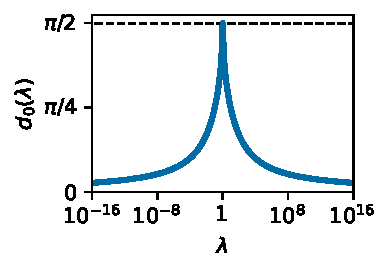
\includegraphics{src/fig-d0lambda.pdf}
    \caption{$d_0(\lmd)$(式\eqref{eq:d0lambda})のグラフ}
    \label{fig:d0lambda}
  \end{figure}

  上述より,$h$が十分小さいとき$\log(A)$に対するDE公式の誤差は最大固有値$\lmdmax$と最小固有値$\lmdmin$のみに依存する.すなわち,
  \begin{align}
    \norm{\log(A) - \sum_{k=-\infty}^\infty h\Fde(kh)}_2
    \le \max_{\lmd\in\{\lmdmax,\lmdmin\}}\left|\log(\lmd)- \sum_{k=-\infty}^\infty h\fde(kh,\lmd)\right|
  \end{align}
  である.
  さらに,$\lmdmax\lmdmin=1$,すなわち,$|\log(\lmdmax)|=|\log(\lmdmin)|$を仮定すると,$d_0(\lmdmax) = d_0(1/\lmdmax) = d_0(\lmdmin)$であることから$\log(\lmdmax)$と$\log(\lmdmin)$に対するDE公式の収束率は等しくなり,\eqref{eq:err_de_sc}より
  \begin{align}
    \norm{\log(A) - \sum_{k=-\infty}^\infty h\Fde(ih)}_2 \le \calO\left(\exp\left(-\frac{2\pi d_0(\lmdmax)}{h}\right)\right) = \calO\left(\exp\left(-\frac{2\pi d_0(\sqrt{\kpp(A)})}{h}\right)\right)
  \end{align}
  となる.
  ここで$\kappa(A)=\|A\|_2\|A^{-1}\|_2$である.
  なお,$\log(A) = \log(pA) - \log(p)I~~(p>0)$が成り立つので,$A$を$pA~~(p=1/\sqrt{\lmdmax\lmdmin})$と定数倍することを考えれば仮定$\lmdmax\lmdmin=1$は一般性を失わない.
  
  さらに,DE公式を計算するための有限の積分区間が$[l,r]$と得られているとする.
  なお,このような区間は文献\cite{tatsuoka_algorithms_2019}におけるAlgorithm 1の第2ステップから第11ステップを用いると得られる\footnote{%
    積分区間決定のアルゴリズム\cite[Alg.\ 1]{tatsuoka_algorithms_2019}はDE変換として$t(x)=\tanh(\sinh(x))$を用いることを前提としているが,アルゴリズムの第10ステップおよび第11ステップにおいて,$l = \asinh(2\atanh(2a-1)/\pi),\ r=\asinh(2\atanh(2b-1)/\pi)$と計算することで,本稿で用いた変数変換$t(x)=\tanh(\frac{\pi}{2}\sinh(x))$に対応できる.
  }.
  このとき,台形則の誤差は積分点数$m=(r-l)/h+1$を用いて
  \begin{align}\label{eq:rate_DE}
    &\norm{\log(A)-\sum_{k=1}^{m-2} h\Fde(l+kh) - \frac{h}{2}\bigl(\Fde(l)+\Fde(r)\bigr)}_2\\
    &\quad \le \calO\left(\exp\left(-\frac{2\pi d_0\bigl(\sqrt{\kpp(A)}\bigr)}{r-l}m\right)\right).
  \end{align}
  と表される.
  以上より,本研究の主結果として,$\log(A)$に対するDE公式の収束率
  \begin{align}\label{eq:conv_rate}
    \calO\left(\exp\left(-\frac{2\pi d_0\bigl(\sqrt{\kpp(A)}\bigr)}{r-l}\right)\right)
  \end{align}
  を得る.

  \subsection{DE公式とGL求積との比較}
  本小節ではDE公式とGL求積の収束の速さを比較する.
  $A$の最大固有値と最小固有値の積が1のとき,どちらの求積法も積分点数に対して指数的に誤差が減少し,その誤差を$\calO(\exp(-\phi m))$と表せる.
  ここで,$\phi$は求積法と$\kappa(A)$のみに依存する定数であり,$\phi$が大きいほど収束が速い.
  DE公式では式\eqref{eq:conv_rate}より
  \begin{align}
    \phi = \frac{2\pi d_0\bigl(\sqrt{\kpp(A)}\bigr)}{r-l},
  \end{align}
  GL求積では
  \begin{align}
    \phi = 2\log\left(\frac{\kappa(A)^{1/4}+1}{\kappa(A)^{1/4}-1}\right)
  \end{align}
  である\cite{fasi_computing_2018}.
  そこで,図 \ref{fig:convspeed}にDE公式とGL求積における収束の速さ$\phi$を$\kappa(A)$に対してプロットしたものを示す.
  なお,DE公式の有限な積分区間$[l,r]$は積分区間決定のアルゴリズム\cite[Alg.\ 1]{tatsuoka_algorithms_2019}を用いて,積分区間の打ち切り誤差が$\eps=2^{-53}\approx 1.1\times 10^{-16}$以下になるように得た\footnote{%
    積分区間決定のアルゴリズム\cite[Alg.\ 1]{tatsuoka_algorithms_2019}は$\|A^{-1}\|_2$,$\|A-I\|_2$,及び$A$のスペクトル半径を必要とするが,$A$が正定値エルミート行列かつ$\lmdmax\lmdmin=1$のときは$\kappa(A)$からその値を求めることができる.したがって本稿では積分区間$[l,r]$は$\kappa(A)$と$\eps$のみに依存する.
  }.
  図 \ref{fig:convspeed}より,$\kpp(A)\gtrsim 2.7 \times 10^3$のときDE公式が速く収束し,$\kpp(A)\lesssim 2.7 \times 10^3$のときGL求積が速く収束することがわかる.
  この結果から,正定値エルミート行列の対数を数値積分法で計算するときには,条件数が大きいときはDE公式,小さいときはGL求積を選べば良いと分かる.

  \begin{figure}[htbp]
    \centering
    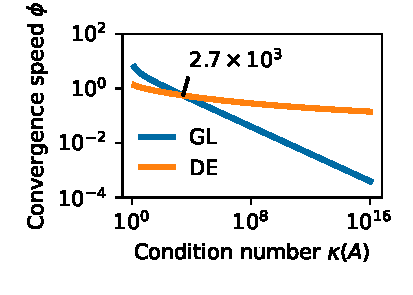
\includegraphics{src/fig-convspeed.pdf}
    \caption{DE公式とGL求積の収束の速さ.$\phi$が大きいほど収束が速い.}
    \label{fig:convspeed}
  \end{figure}

  \section{数値例}
  本節では表 \ref{tab:matrices}に示す行列を用いて,DE公式の収束率の見積りの妥当性を確かめる.
  なお,プログラミングはJuliaを用いて行い,特に明記しない限り倍精度演算を用いた.
  任意精度演算はJuliaの\texttt{BigFloat}型を用いて実装し,GL求積の積分点と重みの計算には\texttt{QuadGK.jl}\footnote{\url{https://github.com/JuliaMath/QuadGK.jl}}を用いた.
  なお,計算に用いたソースコードと実行結果は\url{https://github.com/f-ttok/article-rims2019}にアップロードした.
  \begin{table}[tbp]
    \centering
    \caption{数値例で用いたテスト行列}
    \label{tab:matrices}
    \begin{tabular}{lll}\hline
      行列 & $n$ & $\kpp(A)$\\\hline
      \texttt{nos4} \cite{davis_university_2011} & 100 & $1.6\times 10^3$ \\
      \texttt{bcsstk04} \cite{davis_university_2011} & 132 & $2.3\times 10^6$ \\
      \texttt{lund\_b} \cite{davis_university_2011} & 147 & $3.0\times 10^4$ \\
      \hline
    \end{tabular}
  \end{table}
  計算手順は以下のとおりである.
  \begin{enumerate}
    \item $\tilde{A} = A/\sqrt{\lmdmax\lmdmin}$とスケーリングし,$\log(\tilde{A})$を任意精度演算向きのInverse Scaling and Squaringアルゴリズム\cite[Alg.\ 5.1]{fasi_computing_2018}によって計算した.
    \item $\log(\tilde{A})$を倍精度でDE公式によって計算した.
    \item $\log(\tilde{\lmd}_{\mathrm{max}})~(\tilde{\lmd}_{\mathrm{max}} = \lmdmax/\sqrt{\lmdmax\lmdmin})$をDE公式によって計算した.
    ただし$\log(\tilde{A})$をDE公式で計算したときと同じ積分区間を用いた.
    \item 参考のため,$\log(\tilde{A})$をGL求積を用いて計算した.
  \end{enumerate}
  結果の誤差履歴を図\ref{fig:test}に示す.

  \begin{figure}[tbp]
    \centering
    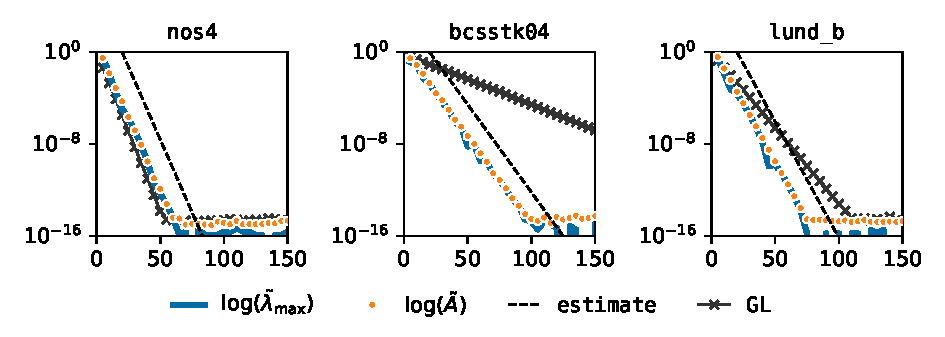
\includegraphics[width=\linewidth]{src/test.pdf}
    \caption{テスト行列に対するDE公式の誤差履歴.}
    \label{fig:test}
  \end{figure}

  図 \ref{fig:test}より以下の3点が観察できた:
  \begin{itemize}
    \item $\lmdmax\lmdmin=1$の条件下では$\log(\tilde{\lmd}_{\mathrm{max}})$と$\log(\tilde{A})$の収束履歴はほぼ一致した.
    \item DE公式の誤差履歴の傾きは,収束率の見積りから得た線の傾きとほぼ一致した.
    \item GL求積とDE公式を比較すると,\texttt{nos4}では同程度の速さで,ほかの2つのテスト行列ではDE公式が速く収束した.これはテスト行列の条件数を考えると妥当な結果である.
  \end{itemize}
  以上より本稿の議論の妥当性を確認できた.


  \section{まとめ}
  本稿では,正定値エルミート行列$A$において,$\log(A)$を計算するためのDE公式の収束率を$A$の条件数をもって見積もった.
  この見積もりを用いてGL求積と比較すると,$A$の条件数が大きいときはDE公式が速く収束し,小さいときはGL求積が速く収束することが分かった.
  条件数の分水嶺の数値はおおよそ$2.7\times 10^3$である.
  また,数値例を通して議論の妥当性を確認した.

  今後の課題として,正定値エルミート行列でない一般の行列に対するGL求積とDE公式の解析が挙げられる.
  また,並列化を行った上で大規模な実問題へ数値積分法を適用し,$\log(A)\bmb$の計算における性能評価を行うことも挙げられる.

  
  \section*{謝辞}
  DE公式の誤差解析についてコメントをいただいた東京大学の田中健一郎先生に感謝申し上げます.
  本研究は日本学術振興会科研費18J22501,18H05392の助成を受けた.

  \bibliography{reference}
  \bibliographystyle{abbrv}
\end{document}
